\labday{29 March 2023}

\experiment{PPDr}

The new laser needed to be aligned since it hit the beamstop in the incorrect place, and did not pass straight through the aperture in the chamber. It was determined at a first glance that the previous alignment system would be unsuitable fo use, since it was locked in place with cyano-threadlocker. The two axes of motion couold be acheived by moving the laser on the screws, and placing shims beneath the laser to raise or lower it in one place.

It was found that the four mounting screws did not leave enough motion to rotate the laser laterally into the correct position. Two screws were removed, and the correct displacement could therefore be acheived. However, at this point, the images provided by PPD were not bright enough, and the laser was still visibly dark. An alignment tool was constructed from 3d printed PLA and a \SI{55}{\micro\metre} fibre, which could be screwed into the scattering chamber and intersect the beam. Figure \ref{fig:PPDFibreScatter} shows the scattering off the fibre, with the camera being triggered by a pulse generator, and the trigger PMT disconnected. The shape of the output seems reasonable, but the intensity of the image is very low, and the laser was visibly dim.

\begin{figure}[H]
\begin{center}
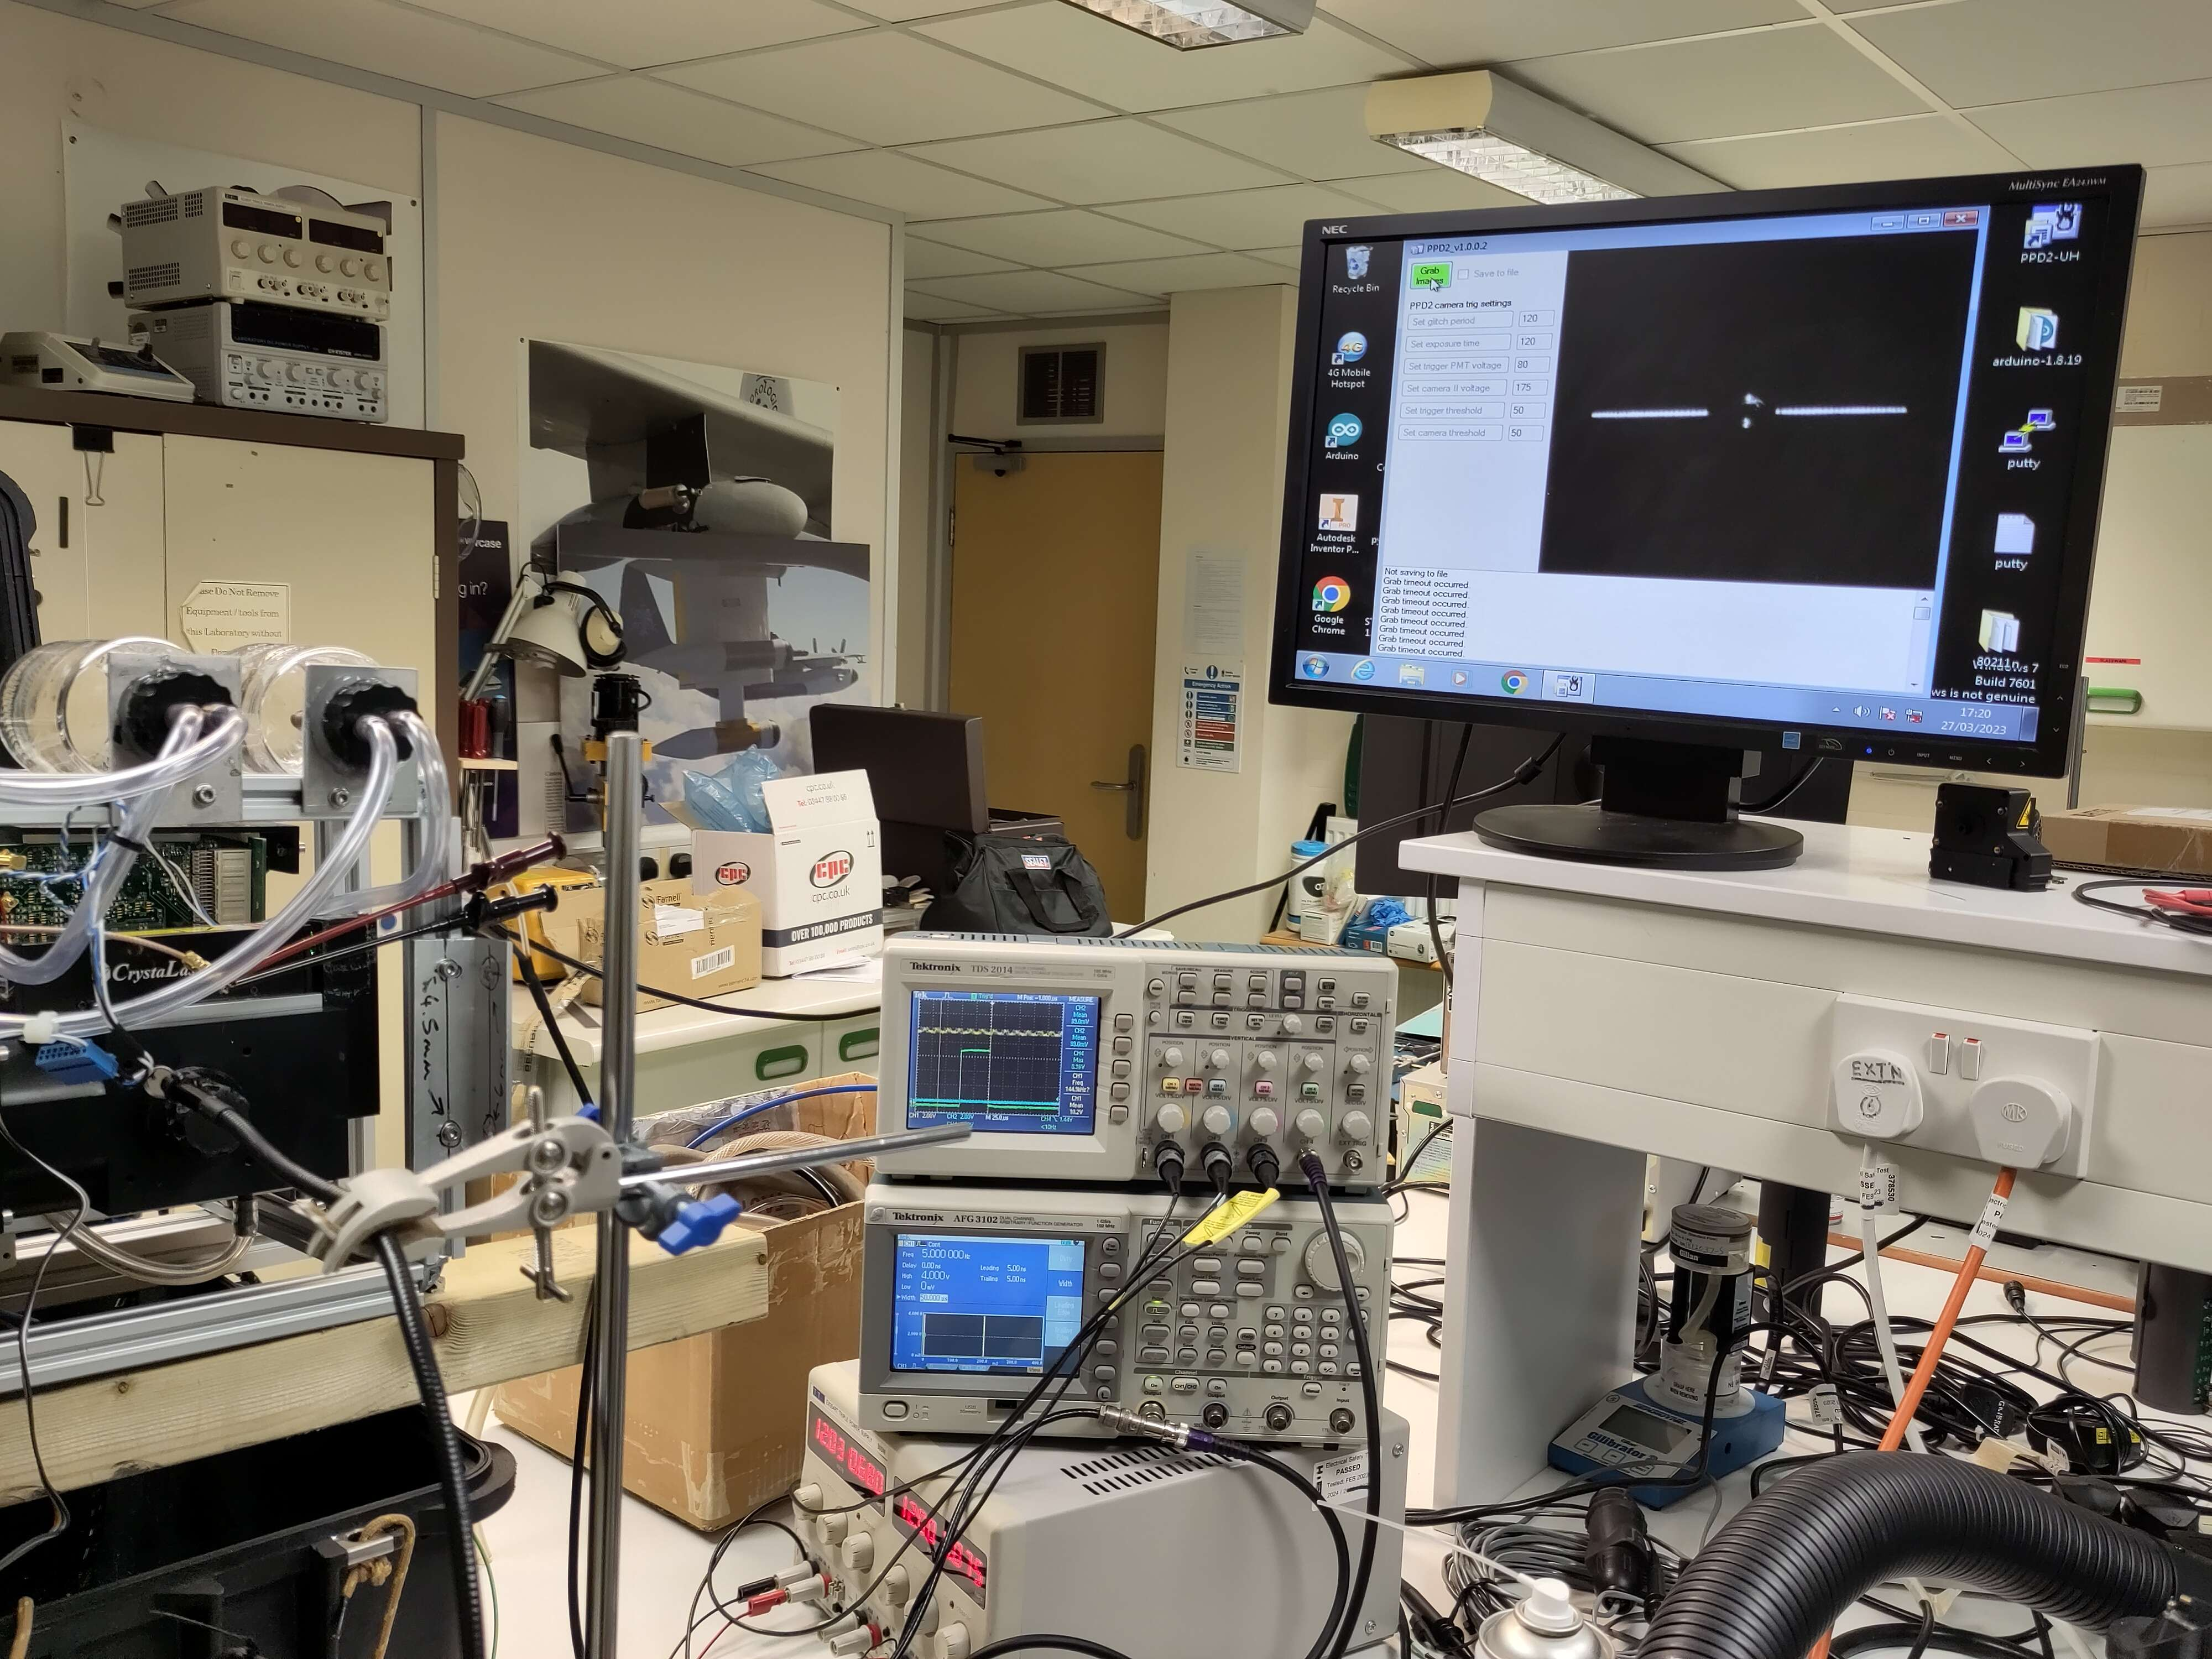
\includegraphics[width=0.5\linewidth]{Figures/PPDFibreScatter}
\end{center}
\caption{Scattering offf fibre tool.}
\label{fig:PPDFibreScatter}
\end{figure}

In order to observe the laser to further dianose issues, a beamview camera was used. The laser was reflected out of the optical block with a mirror, through an OD 2.0 neutral density filter, which lowered the output beam power to below \SI{1}{\milli\watt}, thus making it class 1. The beam appeared extremely low-quality, and looked more like diffraction off the aperture.

When the laser was tilted upwards, the beam quality improved. It was therefore determined that shims needed to be positioned beneath the front of the laser in order to acheive the desired alignment. Tilting of the laser adjusted the position of the beam relative to the aperture. It was determined through trail and improvement that two peices of paper or seven peices of foil were perfect, this is pictured in Fig. \ref{fig:PPDFoilLaser}

\begin{figure}[H]
\begin{center}
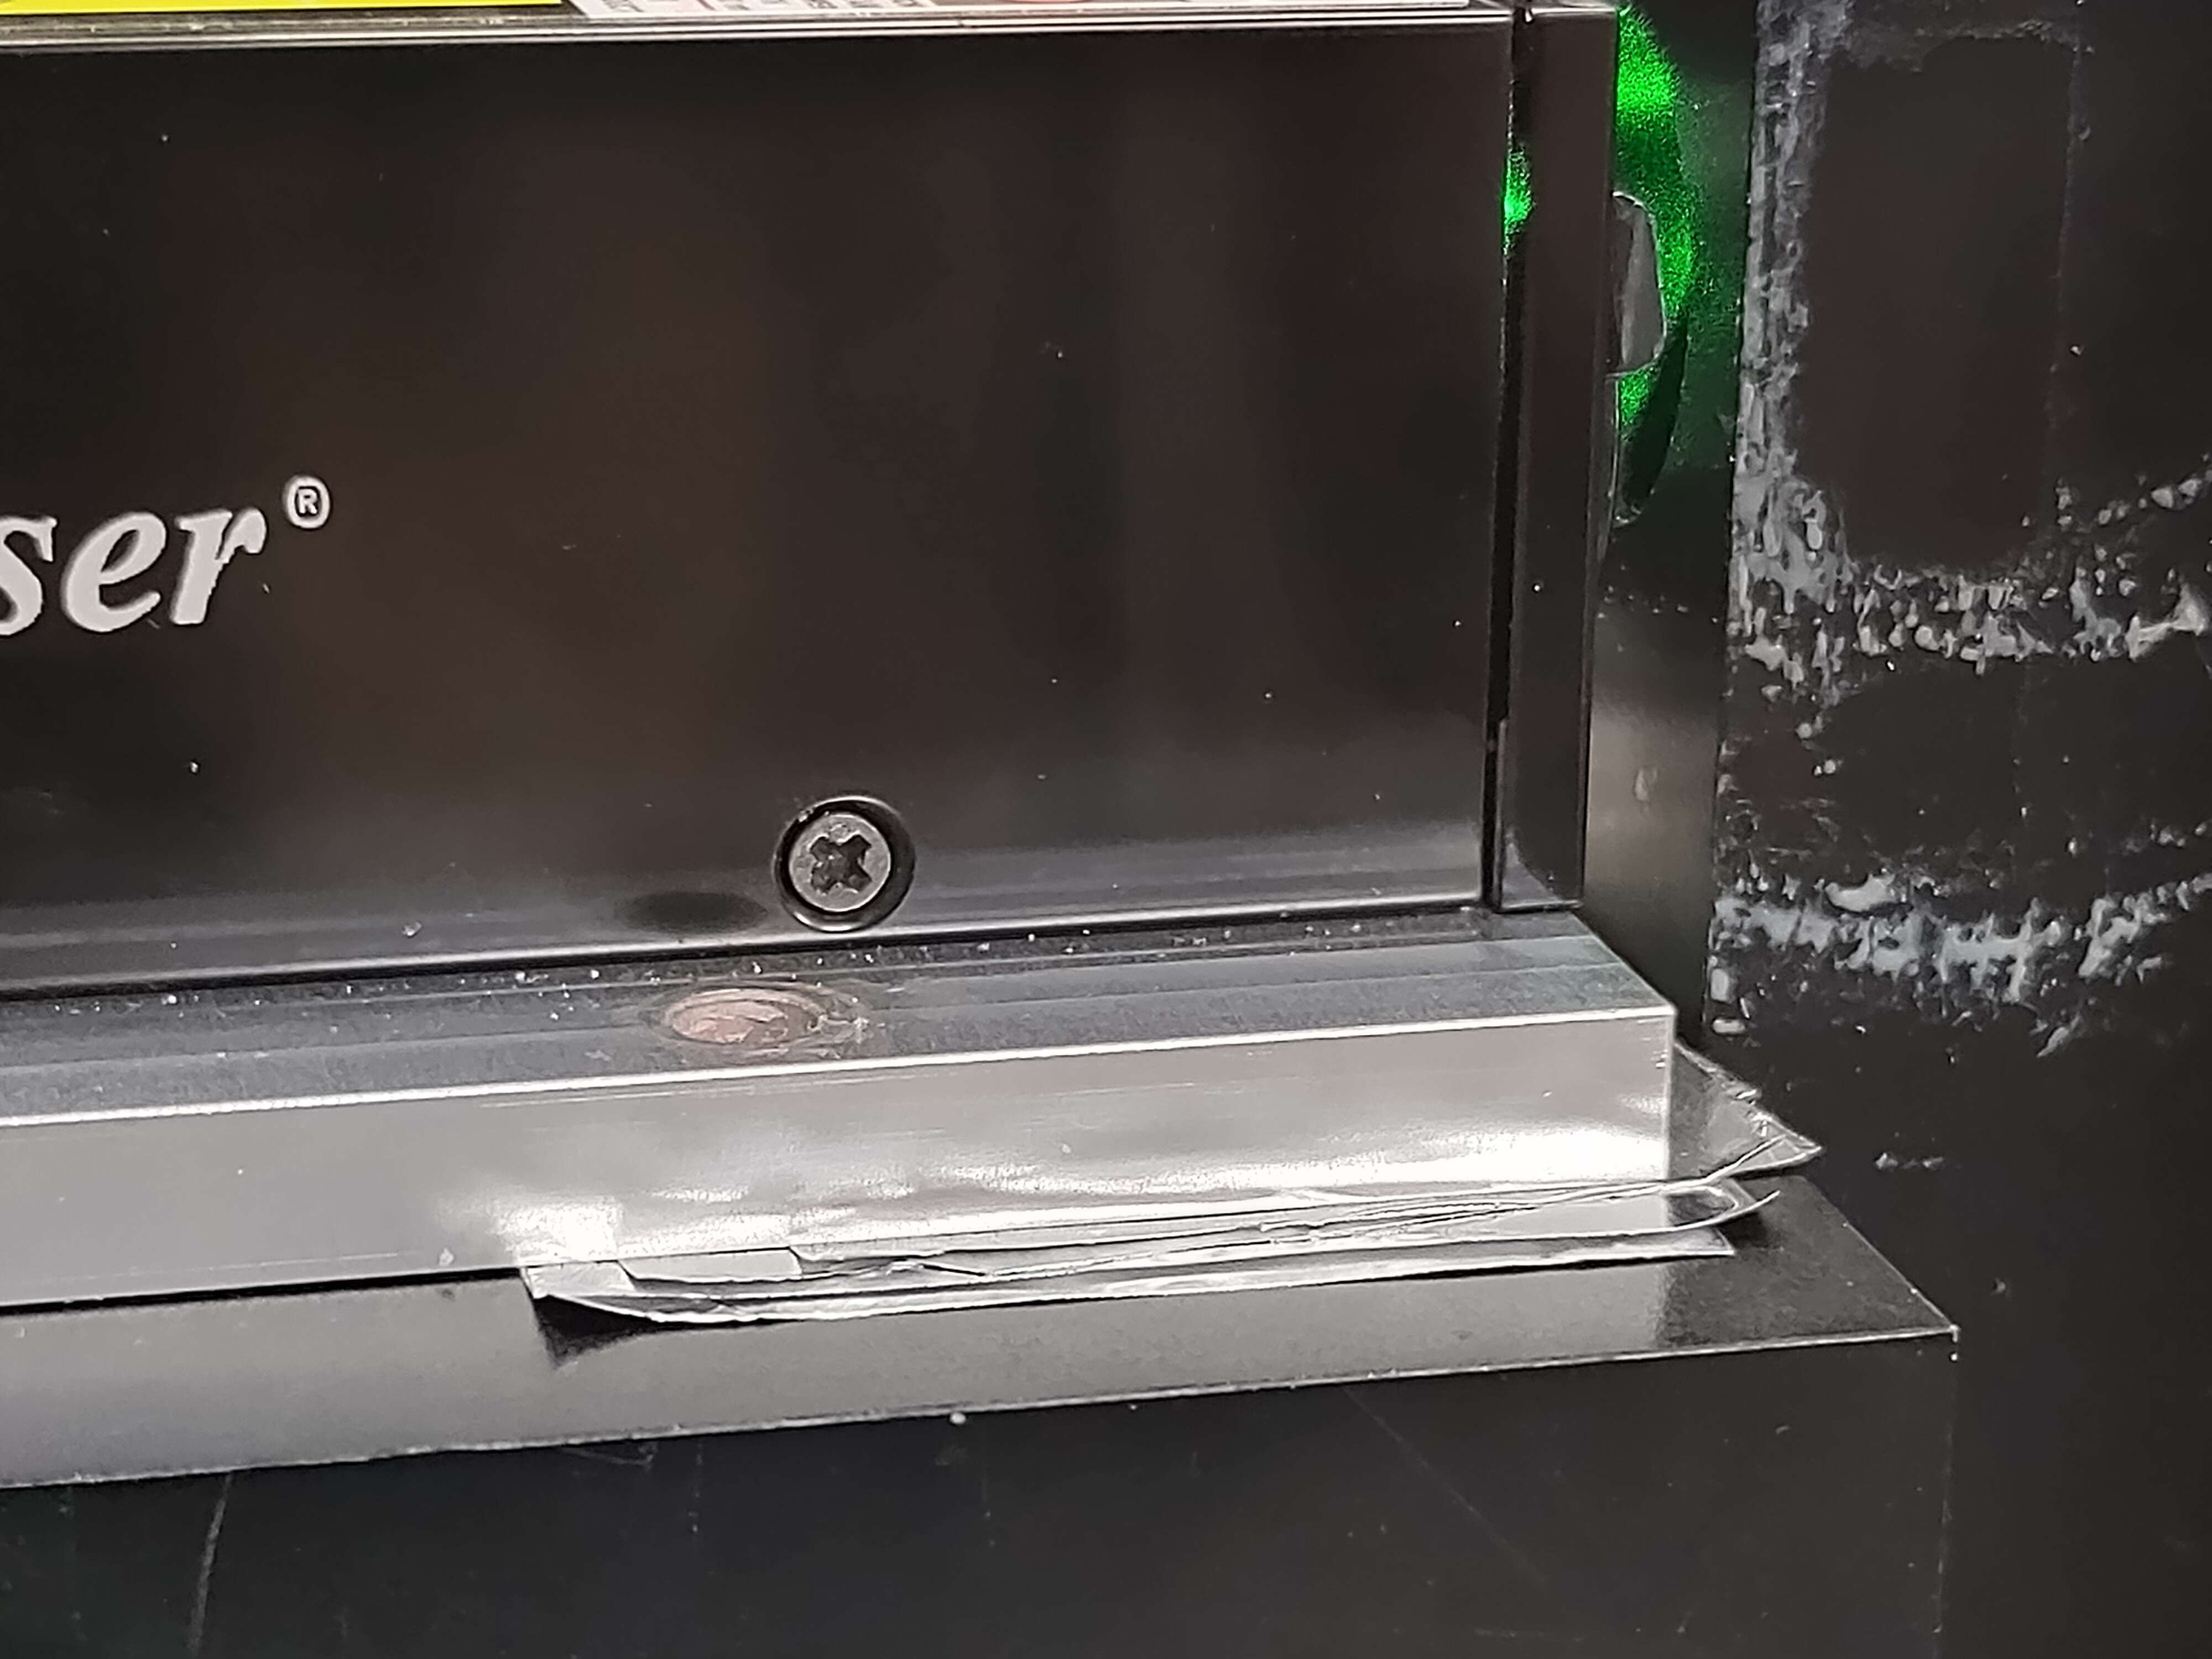
\includegraphics[width=0.5\linewidth]{Figures/PPDFoilLaser}
\end{center}
\caption{Image of foil beneath laser required for alignment.}
\label{fig:PPDFoilLaser}
\end{figure}
